\documentclass[12pt]{article}
\usepackage{mathtools}
\usepackage{amssymb}
\usepackage{amsthm}
\usepackage{polski}
\usepackage[utf8]{inputenc}
\usepackage{geometry}
\usepackage{mnsymbol}
\usepackage{graphicx}
\usepackage{textgreek}
\usepackage{float}
\usepackage{caption}
\author{Łukasz Jezapkowicz}
\title{Generator relaksacyjny}
\date{03.06.2019}
\begin{document}
\newgeometry{tmargin=2cm,bmargin=2cm,lmargin=2cm,rmargin=2cm}
\maketitle
\tableofcontents \newpage
\section{Generator relaksacyjny z wzmacniaczem operacyjnym}
\subsection{Cel ćwiczenia}
Celem ćwiczenia było zapoznanie się z generatorem relaksacyjnym astabilnym z wzmacniaczem operacyjnym oraz zbadanie od czego zależy częstotliwość sygnału wyjściowego.
\subsection{Przebieg ćwiczenia}
Na pulpicie symulacyjnym zbudowałem obwód generatora relaksacyjnego astabilnego z wzmacniaczem operacyjnym widoczny na \textbf{Rys. 1}. Wejście odwracające sterowane jest napięciem z kondensatora $C_1$, natomiast na jego wyjście nieodwracające podawany jest sygnał z dzielnika napięciowego $R_1$,$R_2$ zasilanego napięciem wyjściowym wzmacniacza. Obwód składa się dwóch źródeł napięcia stałego $V_1=12V$,$V_2=12V$, trzech rezystorów $R_1=5k\Omega$,$R_2=10k\Omega$,$R_3=1k\Omega$, kondensatora $C_1=2nF$ oraz wzmacniacza operacyjnego $LM715CH$. Do układu podłączyłem również oscyloskop $XSC1$.
\begin{figure}[H]
\centering
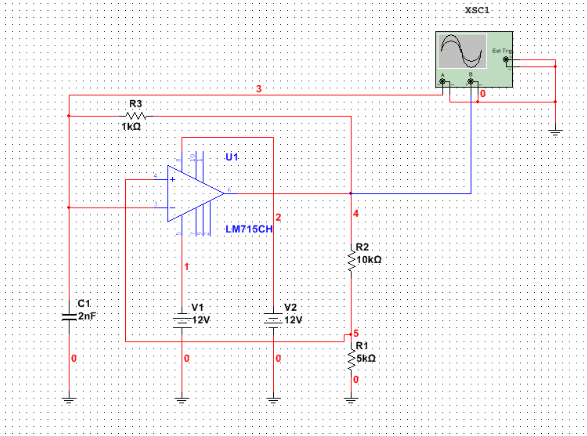
\includegraphics[width=15cm]{1}
\caption*{\textbf{Rys. 1}: Schemat obwodu generatora relaksacyjnego astabilnego z wzmacniaczem operacyjnym }
\end{figure}
\noindent Podczas włączania obwodu kondensator jest rozładowany i na wejście odwracające podawane jest napięcie $0V$ zaś na wyjściu mamy maksymalny sygnał $U_{Z+}$. Kondensator zaczyna się ładować poprzez rezystor $R_3$. Gdy napięcie na wejściu odwracającym i wejściu nieodwracającym zrównają się, napięcie
na wyjściu wzmacniacza zmieni się na maksymalny ujemny sygnał $U_{Z-}$. Od tego momentu kondensator zaczyna się rozładowywać od napięcia $U_{P1}=U_{Z+}\frac{R_1}{R_1+R_2}$ do napięcia $U_{P2}=U_{Z-}\frac{R_1}{R_1+R_2}$. Gdy osiągnie napięcie $U_{P2}$ to napięcie na wyjściu przełącza się z powrotem do
$U_{Z+}$ i całość powtarza się cyklicznie. Na wyjściu mamy sygnał prostokątny widoczny na \textbf{Rys. 2}.
\begin{figure}[H]
\centering
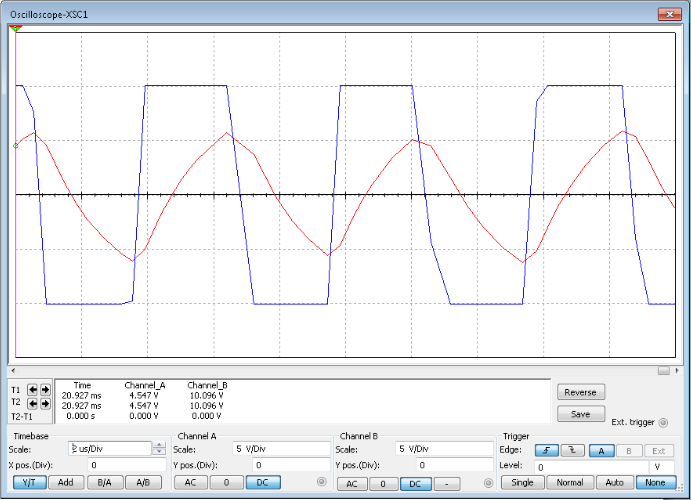
\includegraphics[width=15cm]{2}
\caption*{\textbf{Rys. 2}: Ekran oscyloskopu dla obwodu z Rys. 1. Sygnał wyjściowy zaznaczony jest kolorem niebieskim zaś sygnał na kondensatorze kolorem czerwonym. }
\end{figure}
\noindent Następnie w miejsce rezystora $R_1$ wstawiłem potencjometr $P_1$, którego rezystancja może zmieniać się w zakresie do $40k\Omega$. Zbadałem jak zmienia się częstotliwość $f$ sygnału wyjściowego w zależności od oporu $P_1$. Do pomiaru częstotliwości wykorzystałem miernik częstotliwości $XFC1$ dołączony do wyjścia obwodu. Zmierzyłem częstotliwość dla $P_1$ równego kolejno $5k\Omega$,$10k\Omega$,$20k\Omega$,$40k\Omega$. Na \textbf{Rys. 3} zamieściłem przebieg sygnału wyjściowego dla wartości oporu $5k\Omega$.
Wyniki pomiarów widać w tabeli na \textbf{Rys. 4}. Z pomiarów wynika, że ze wzrostem oporu $P_1$ (wzrostem napięcia z dzielnika) napięcie na kondensatorze też rośnie, zaś częstotliwość maleje.
\begin{figure}[H]
\centering
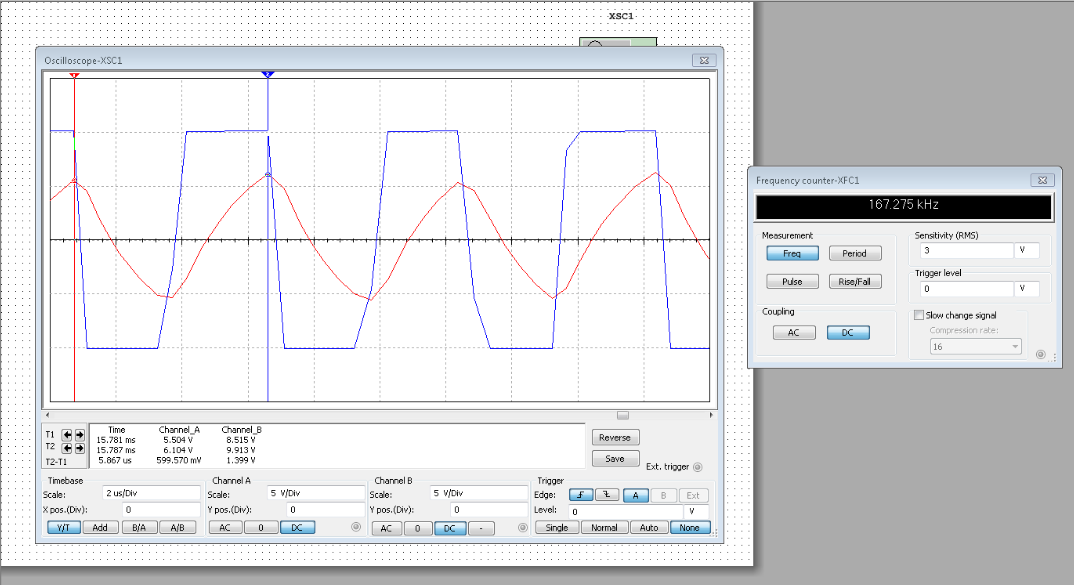
\includegraphics[width=15cm]{3}
\caption*{\textbf{Rys. 3}: Przebieg sygnału wyjściowego dla oporu $P_1=5k\Omega$ }
\end{figure}
\begin{figure}[H]
\centering
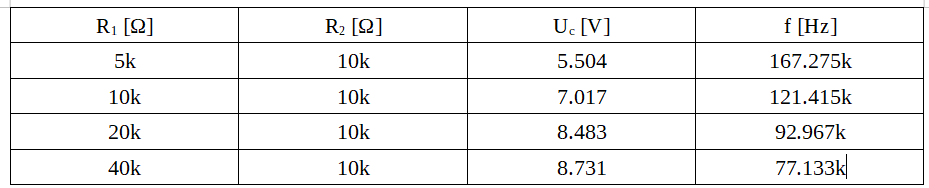
\includegraphics[width=15cm]{4}
\caption*{\textbf{Rys. 4}: Tabela zmierzonych wartości dla różnych wartości $P_1$ }
\end{figure}
\noindent Następnie w miejsce rezystora $R_3$ wstawiłem potencjometr $P_3$, którego rezystancja może zmieniać się w zakresie do $20k\Omega$. Zbadałem jak zmienia się częstotliwość $f$ sygnału wyjściowego w zależności od oporu $P_3$. Opory $R_1$ i $R_2$ ustawiłem na odpowiednio $5k\Omega$ oraz $10k\Omega$. Zmierzyłem częstotliwość dla $P_3$ równego kolejno $1k\Omega$,$5k\Omega$,$10k\Omega$,$20k\Omega$. Na \textbf{Rys. 5} zamieściłem przebieg sygnału wyjściowego dla wartości oporu $1k\Omega$. Wyniki pomiarów widać w tabeli na \textbf{Rys. 6}. Z pomiarów wynika, że ze wzrostem oporu $P_3$ napięcie na kondensatorze maleje, zaś częstotliwość rośnie.
\begin{figure}[H]
\centering
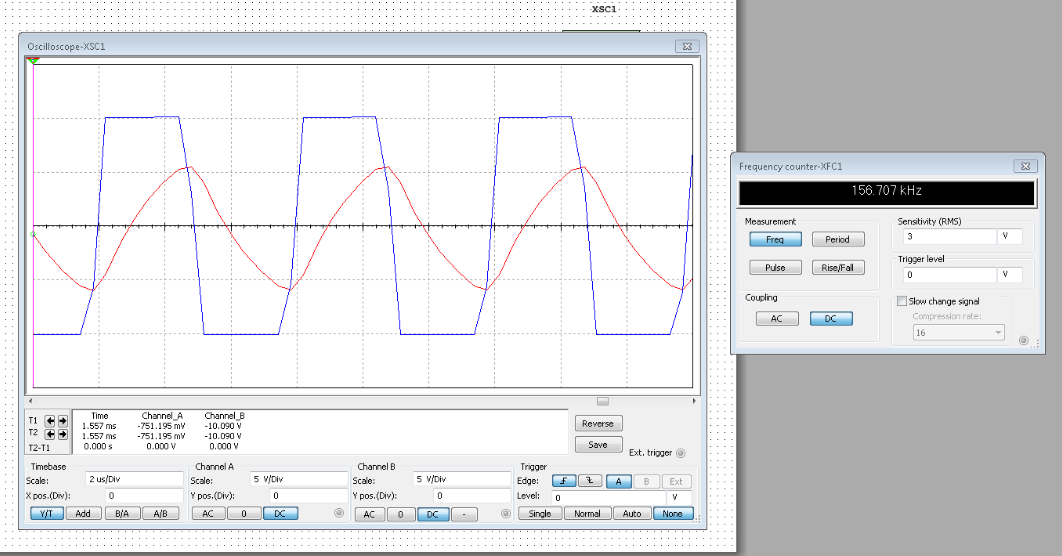
\includegraphics[width=15cm]{5}
\caption*{\textbf{Rys. 5}: Przebieg sygnału wyjściowego dla oporu $P_3=1k\Omega$ }
\end{figure}
\begin{figure}[H]
\centering
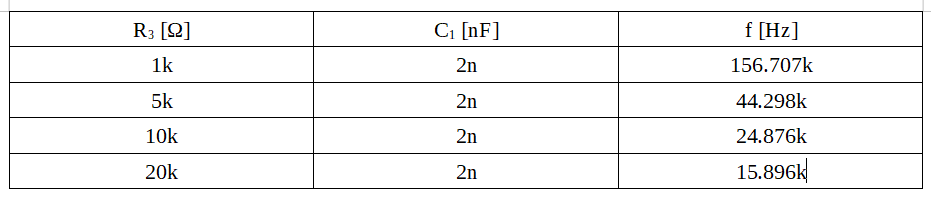
\includegraphics[width=15cm]{6}
\caption*{\textbf{Rys. 6}: Tabela zmierzonych wartości dla różnych wartości $P_3$ }
\end{figure}
\noindent Następnie dla $R_1=5k\Omega$,$R_2=10k\Omega$,$R_3=1k\Omega$ zbadałem wpływ zmian pojemności kondensatora na częstotliwość $f$. Zmierzyłem częstotliwość dla $C_1$ równego kolejno $2nF$,$5nF$,$10nF$,$20nF$.  Na \textbf{Rys. 7} zamieściłem przebieg sygnału wyjściowego dla pojemności $2nF$. Wyniki pomiarów widać w tabeli na \textbf{Rys. 8}. Z pomiarów wynika, że ze wzrostem pojemności $C_1$ napięcie na kondensatorze rośnie, zaś częstotliwość maleje.
\begin{figure}[H]
\centering
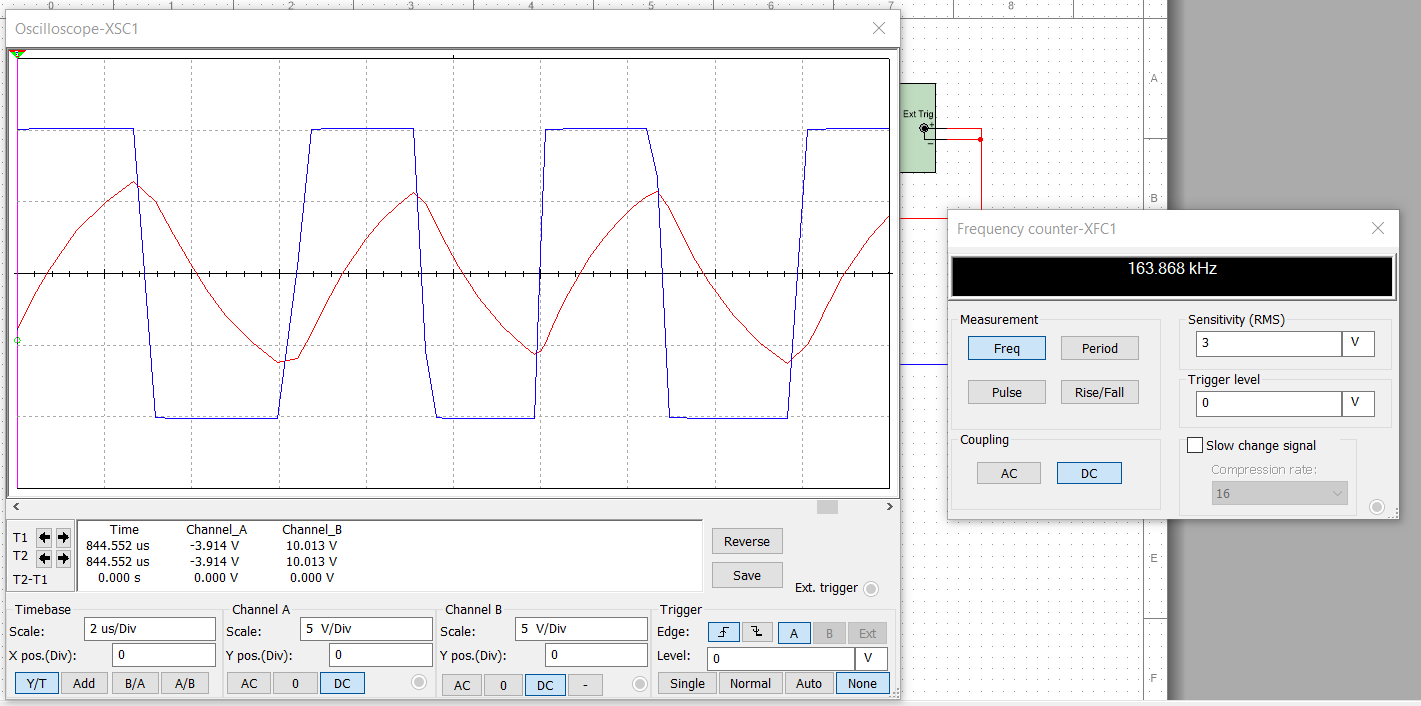
\includegraphics[width=15cm]{7}
\caption*{\textbf{Rys. 7}: Przebieg sygnału wyjściowego dla pojemności $C_1=2nF$ }
\end{figure}
\begin{figure}[H]
\centering
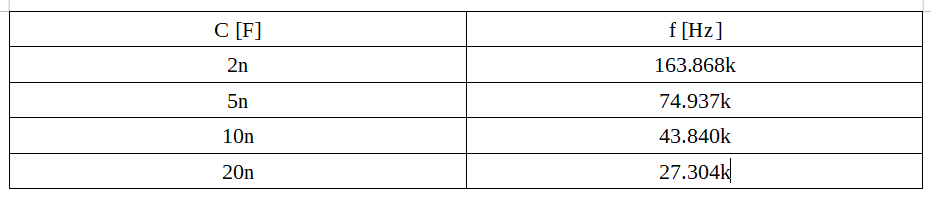
\includegraphics[width=15cm]{8}
\caption*{\textbf{Rys. 8}: Tabela zmierzonych wartości dla różnych wartości $C_1$ }
\end{figure}
\subsection{Wnioski}
Wykonane ćwiczenie pozwala wyciągnąć wnioski na temat wartości częstotliwości $f$ sygnału wyjściowego. Częstotliwość ta wraz ze wzrostem napięcia na kondensatorze maleje czyli czym większe napięcie z dzielnika napięcia (wzrost $R_1$) tym mniejsza częstotliwość $f$. Natomiast wraz ze spadkiem napięcia na kondensatorze częstotliwość $f$ rośnie czyli czym większy opór $R_3$ tym większa częstotliwość. Częstotliwość $f$ wraz ze wzrostem pojemności $C_1$ maleje, ponieważ wzrost pojemności oznacza wzrost napięcia na kondensatorze. Częstotliwość w naszym obwodzie z \textbf{Rys. 1} zależy więc od $R_1$,$R_2$,$R_3$,$C_1$.
\section{Generator relaksacyjny z dwoma progami komparacji}
\subsection{Cel ćwiczenia}
Celem ćwiczenia było zapoznanie się z generatorem relaksacyjnym z dwoma progami komparacji oraz zbadanie jak $U_{P1}$,$U_{P2}$ oraz częstotliwość $f$ zależą od oporu $R_{12}$ (napięcia na kondensatorze).
\subsection{Przebieg ćwiczenia}
Na pulpicie symulacyjnym zbudowałem obwód generatora relaksacyjnego z dwoma progami komparacji widoczny na \textbf{Rys. 9}. Obwód składa się źródła napięcia stałego $V_1=5V$, trzech rezystorów $R_{11}=1k\Omega$,$R_{13}=1k\Omega$,$R_3=1k\Omega$, potencjometru
$R_{12}=1k\Omega$, kondensatora $C_1=100nF$, dwóch komparatorów $U_1$,$U_2$ oraz przerzutnika $RS$. Do układu podłączyłem również oscyloskop $XSC1$ i miernik częstotliwości $XFC1$.
\begin{figure}[H]
\centering
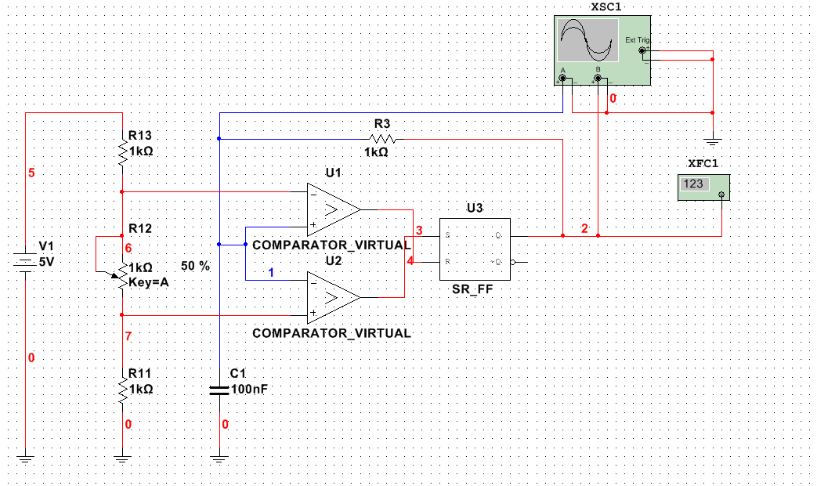
\includegraphics[width=15cm]{9}
\caption*{\textbf{Rys. 9}: Schemat obwodu generatora relaksacyjnego z dwoma progami komparacji }
\end{figure}
\noindent Przerzutnik $RS$ posiada dwa wejścia S (Set) oraz R (Reset) a także dwa wyjścia Q oraz ~Q. Przerzutnik jest urządzeniem dwustanowym więc na jego wyjściu może pojawić się sygnał wysoki (1) lub niski (0) w zależności od kombinacji sygnałów wejściowych. Na przykład gdy na wejściu S pojawia się sygnał wysoki (1) a na wejściu R niski (0) to na wyjściu Q pojawia się sygnał wysoki (1). Sygnał wyjściowy jest sygnałem prostokątnym widocznym na \textbf{Rys. 10}.
\begin{figure}[H]
\centering
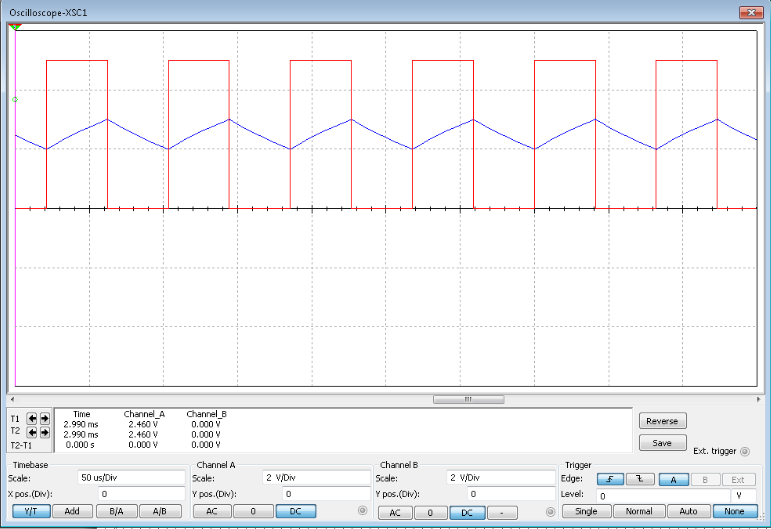
\includegraphics[width=15cm]{10}
\caption*{\textbf{Rys. 10}: Ekran oscyloskopu dla obwodu z Rys. 9. Sygnał wyjściowy zaznaczony jest kolorem czerwonym zaś sygnał na kondensatorze kolorem niebieskim. }
\end{figure}
\noindent Do obwodu podłączyłem dwa multimetry pozwalające zmierzyć napięcia progowe wyzwalające oba komparatory ($U_{P1}$,$U_{P2}$). Zbadałem zmianę częstotliwości $f$ w zależności od od zmiany oporu $R_{12}$. Zmierzyłem częstotliwość dla $R_{12}$ równego kolejno
$0.25k\Omega$,$0.5k\Omega$,$0.75k\Omega$,$1k\Omega$. Na \textbf{Rys. 11} zamieściłem przebieg sygnału wyjściowego dla oporu $R_{12}=1k\Omega$. Wyniki pomiarów widać w tabeli na \textbf{Rys. 12}. Z pomiarów wynika, że ze wzrostem oporu $R_{12}$ (czyli wzrostem napięcia na kondensatorze) napięcie $U_{P1}$ rośnie, $U_{P2}$ maleje, zaś częstotliwość $f$ maleje.
\begin{figure}[H]
\centering
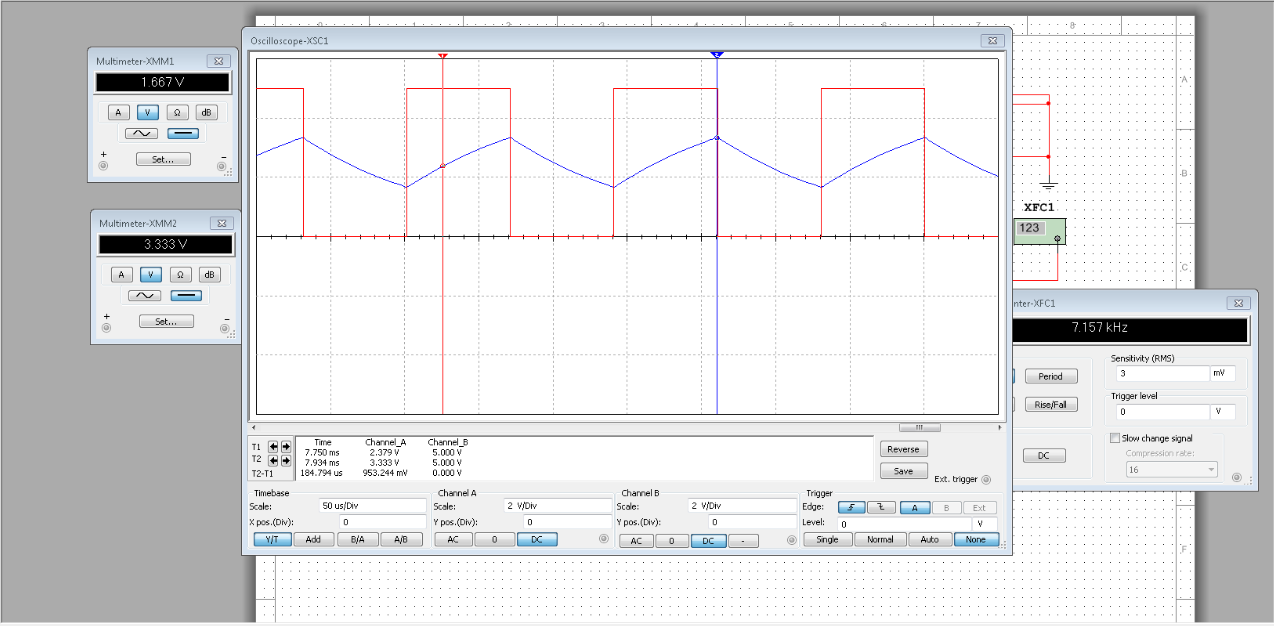
\includegraphics[width=15cm]{11}
\caption*{\textbf{Rys. 11}: Przebieg sygnału wyjściowego dla oporu $R_{12}=1k\Omega$ }
\end{figure}
\begin{figure}[H]
\centering
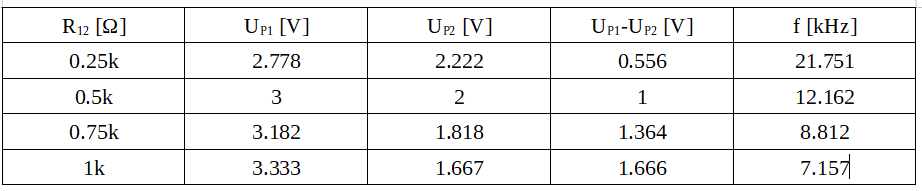
\includegraphics[width=15cm]{12}
\caption*{\textbf{Rys. 12}: Tabela zmierzonych wartości dla różnych wartości $R_{12}$ }
\end{figure}
\subsection{Wnioski}
Wykonane ćwiczenie pozwala wyciągnąć wnioski na temat wartości częstotliwości $f$ sygnału wyjściowego oraz wartości napięć progowych $U_{P1}$,$U_{P2}$. Napięcia progowe $U_{P1}$,$U_{P2}$ w naszym obwodzie z \textbf{Rys. 9} zależą od napięcia na dzielniku napięciowym czyli od $R_{11}$,$R_{12}$,$R_{13}$. Częstotliwość sygnału wyjściowego $f$ wraz ze wzrostem $R_{12}$ maleje.
\section{Generator sterowany napięciem VCO (Voltage Controlled Oscillator)}
\subsection{Cel ćwiczenia}
Celem ćwiczenia było zapoznanie się z generatorem sterowanym napięciem VCO (Voltage Controlled Oscillator) oraz zaobserwowanie przebiegu na kondensatorze i wyjściowego układu.
\subsection{Przebieg ćwiczenia}
Na pulpicie symulacyjnym zbudowałem obwód generatora sterowanego napięciem VCO widoczny na \textbf{Rys. 13}. Obwód składa się źródła napięcia stałego $V_1=4V$, rezystora $R_3=1k\Omega$, kondensatora $C_1=20nF$, dwóch komparatorów $U_1$,$U_2$ oraz przerzutnika $RS$. Do układu podłączyłem również oscyloskop $XSC1$, miernik częstotliwości $XFC1$ oraz generator $XFG1$ wytwarzający sygnał sinusoidalny o parametrach: częstotliwość $50Hz$ oraz amplituda $1V$.
\begin{figure}[H]
\centering
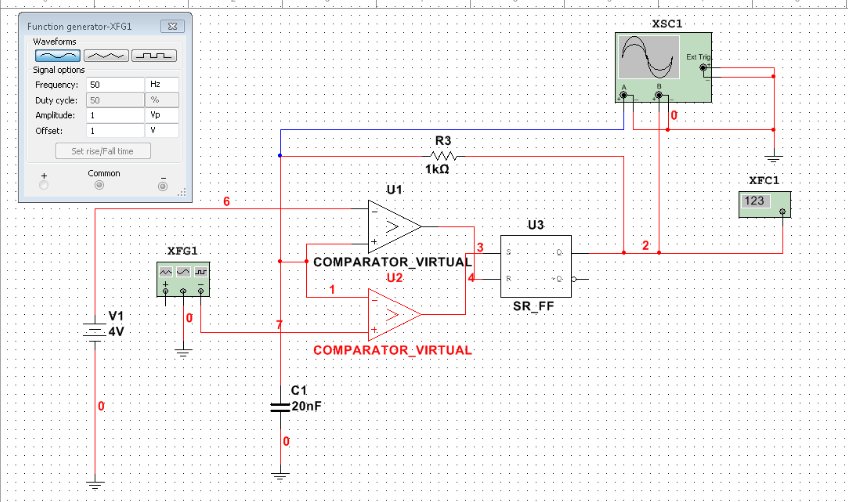
\includegraphics[width=15cm]{13}
\caption*{\textbf{Rys. 13}: Schemat obwodu generatora sterowanego napięciem VCO }
\end{figure}
\noindent Generator ten to typ generatora, w którym częstotliwość oscylacji wyjściowych zmienia się wraz ze zmianą amplitudy sygnału wejściowego. Zbudowany jest na bazie generatora astabilnego z dwoma komparatorami. Na wejście nieodwracające dolnego komparatora podany jest sygnał sinusoidalny z generatora, który ustala zmienny dolny próg przełączania $U_{P1}$. Na wejście odwracające górnego komparatora wprowadzone zostało stałe napięcie, które ustala górny próg przełączania $U_{P2}$. Zmienny dolny próg przełączania sprawia, że sygnał wyjściowy raz jest "gęstszy" i ma większą częstotliwość (co zostało ukazane na \textbf{Rys. 13}) zaś innym razem jest "rzadszy" i ma mniejszą częstotliwość (co zostało ukazane na \textbf{Rys. 14}).
\begin{figure}[H]
\centering
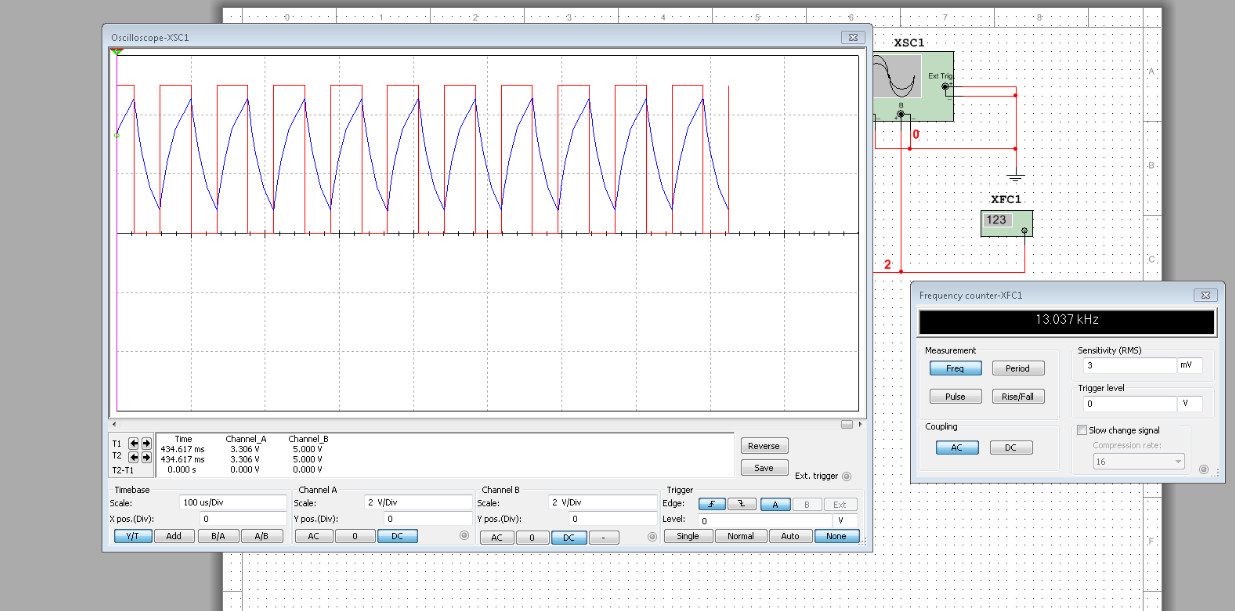
\includegraphics[width=15cm]{14}
\caption*{\textbf{Rys. 14}: Ekran oscyloskopu dla obwodu z Rys. 13. Sygnał wyjściowy jest "gęstszy" i częstotliwość jest duża ($13.037kHz$) }
\end{figure}
\begin{figure}[H]
\centering
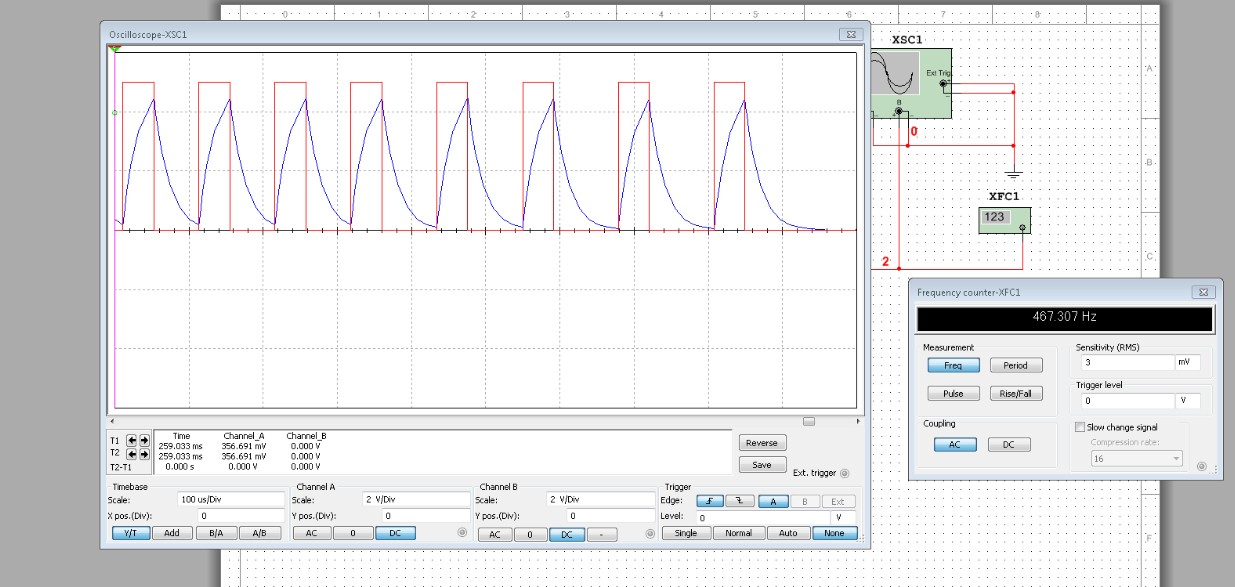
\includegraphics[width=15cm]{15}
\caption*{\textbf{Rys. 15}: Ekran oscyloskopu dla obwodu z Rys. 13. Sygnał wyjściowy jest "rzadszy" i częstotliwość jest mała ($467.307Hz$) }
\end{figure}
\subsection{Wnioski}
Wykonane ćwiczenie pozwala wyciągnać wnioski na temat wartości częstotliwości $f$ sygnału wyjściowego. Gdy na wejście nieodwracające dolnego komparatora podany jest sygnał sinusoidalny z dużą amplitudą to sygnał wyjściowy jest "rzadszy" i częstotliwość jest mniejsza, zaś gdy 
podany jest sygnał sinusoidalny z małą amplitudą to sygnał wyjściowy jest "gęstszy" i częstotliwość jest większa.
\end{document}
